\chapter{Migración}

\section{Proyecto}
El Punto de vista de Proyecto se utiliza principalmente para modelar la gestión del cambio de arquitectura. La arquitectura del proceso de migración de una vieja situación (estado actual Arquitectura empresarial) a una nueva situación deseada (estado objetivo arquitectura empresarial) tiene consecuencias importantes en el proceso de toma de decisiones posteriores de la estrategia de crecimiento a largo plazo y mediano plazo. \cite{ArchiMat55:online} \vspace{\baselineskip}

El Punto de vista de Proyecto plasma la gestión del cambio de arquitectura y actores involucrados, detalla el objetivo de la aplicación.

\subsection{Modelo}
\begin{figure}[h!]
	\centering
	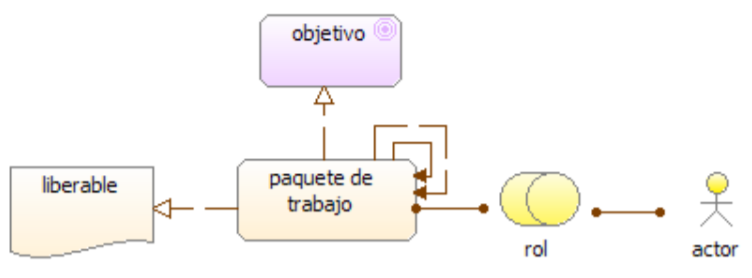
\includegraphics[width=0.8\linewidth]{Arquitectura/Migracion/imgs/ProyectoMetamodelo.PNG}
	\caption{Modelo:  Proyecto}
\end{figure}
\newpage
\subsection{Caso de Estudio}
\begin{figure}[h!]
	\centering
	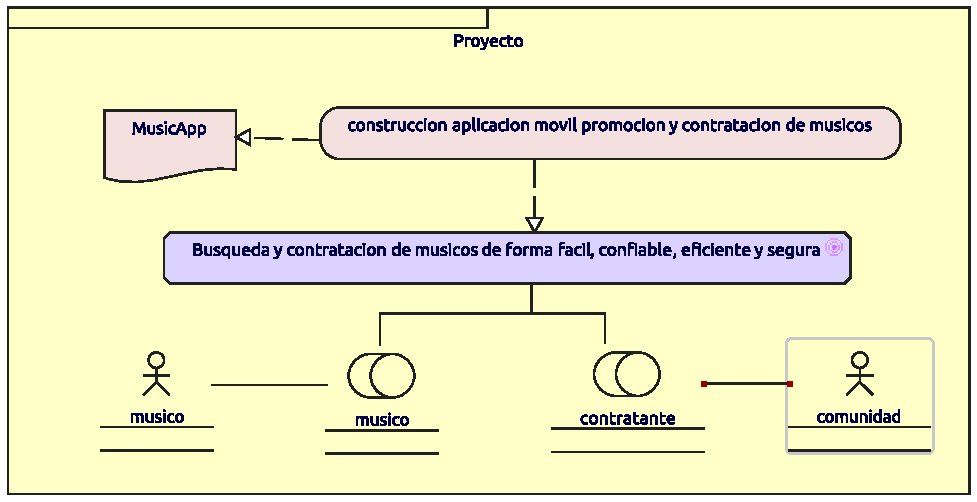
\includegraphics[width=\linewidth]{Arquitectura/Migracion/imgs/Proyecto.pdf}
	\caption{Caso de estudio: Proyecto}
	\label{fig:comportamiento}
\end{figure}

\newpage

\section{Migración}
El Punto de vista de Migración implica modelos y conceptos que se pueden utilizar para especificar la transición de una arquitectura existente a una arquitectura deseada. \cite{ArchiMat55:online} \vspace{\baselineskip}


\subsection{Modelo}
\begin{figure}[h!]
	\centering
	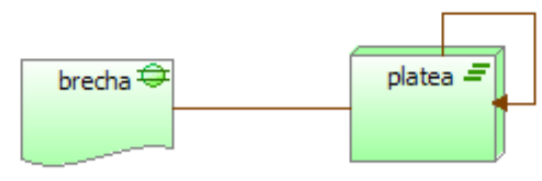
\includegraphics[width=0.8\linewidth]{Arquitectura/Migracion/imgs/MigracionMetamodelo.PNG}
	\caption{Modelo:  Migración}
\end{figure}
\newpage
\subsection{Caso de Estudio}
\begin{figure}[h!]
	\centering
	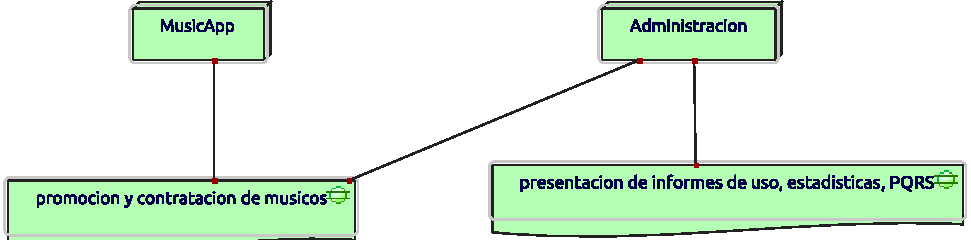
\includegraphics[width=\linewidth]{Arquitectura/Migracion/imgs/Migracion.pdf}
	\caption{Caso de estudio: Migración}
	\label{fig:comportamiento}
\end{figure}

\newpage

\section{Migración e Implementación}
El Punto de vista de Migración e Implementación se utiliza para relacionar los programas y proyectos de las partes de la arquitectura que se implementan. Esta vista permite el modelado del alcance de los programas, proyectos, actividades del proyecto en términos de las mesetas que se realizan o los elementos de la arquitectura individuales que se ven afectados. Además, la forma en que se ven afectados los elementos puede ser indicado por la anotación de las relaciones. \cite{ArchiMat55:online} \vspace{\baselineskip}

El siguiente modelo muestra la relación del prototipo de la aplicación y el proyecto generado, involucra la arquitectura y la relación con los usuarios.

\subsection{Modelo}
\begin{figure}[h!]
	\centering
	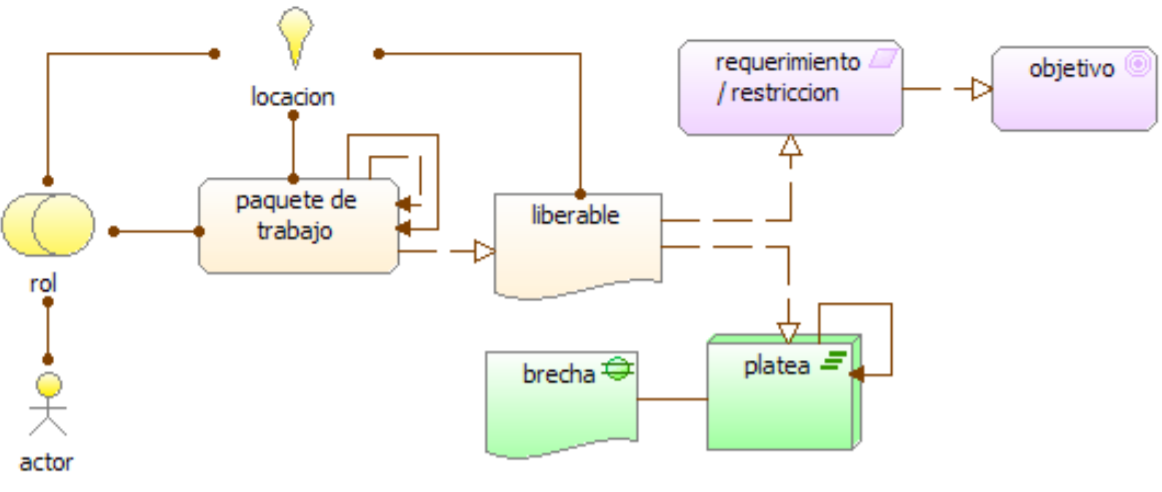
\includegraphics[width=\linewidth]{Arquitectura/Migracion/imgs/MigracionImplementacionMetamodelo.PNG}
	\caption{Modelo: Migración e Implementación}
\end{figure}
\newpage
\subsection{Caso de Estudio}
\begin{figure}[h!]
	\centering
	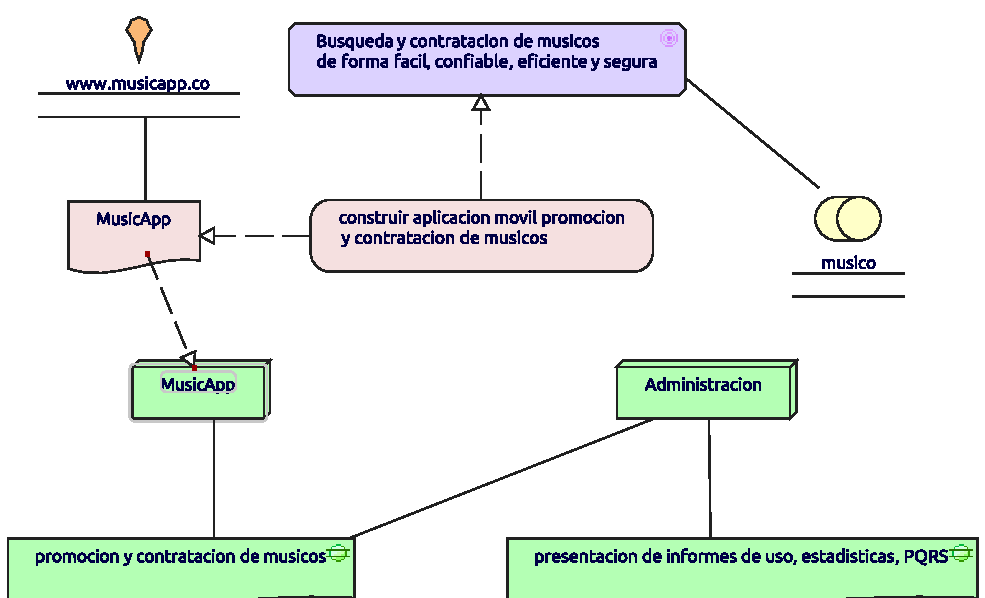
\includegraphics[width=\linewidth]{Arquitectura/Migracion/imgs/MigracionImplementacion.pdf}
	\caption{Caso de estudio: Migración e Implementación}
	\label{fig:comportamiento}
\end{figure}

\newpage